\documentclass[border=10pt]{standalone}
\usepackage{tikz}
\usetikzlibrary{positioning}
\begin{document}
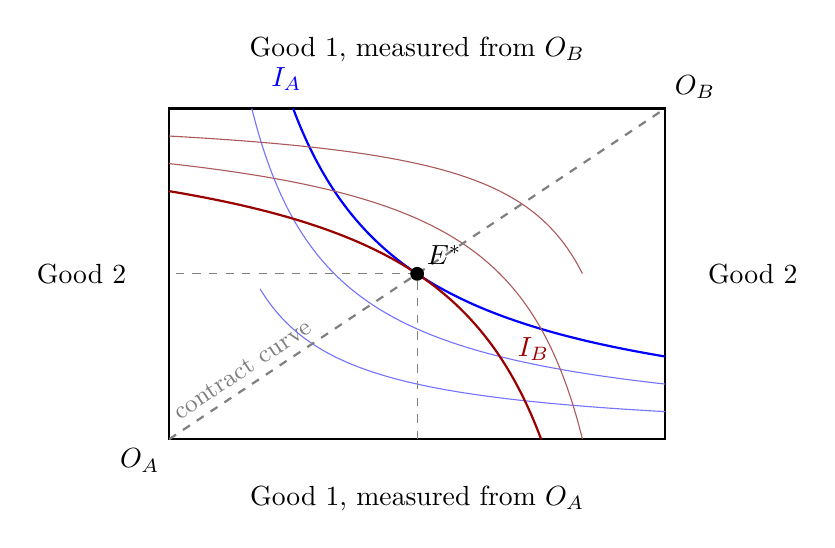
\begin{tikzpicture}[x=1.05cm, y=1.05cm]
  % box
  \draw[thick] (0,0) -- (6,0) -- (6,4) -- (0,4) -- cycle;
  \begin{scope}
    \clip (0,0) -- (6,0) -- (6,4) -- (0,4) -- cycle;
    % A's indifference curves (convex toward O_A at bottom-left)
    \draw[blue!55] plot[domain=1.1:6.5, samples=100, smooth] (\x, {2/\x});
    \draw[blue!55] plot[domain=1:6.5, samples=100, smooth] (\x, {4/\x});
    \draw[blue, thick] plot[domain=1.5:6.5, samples=100, smooth] (\x, {6/\x});
    % B's indifference curves (convex toward O_B at top-right), clipped to box
    \draw[red!50!black!65] plot[domain=0:5, samples=80, smooth] (\x, {4 - 2/(6-\x)});
    \draw[red!50!black!65] plot[domain=0:5, samples=80, smooth] (\x, {4 - 4/(6-\x)});
    \draw[red!60!black, thick] plot[domain=0:4.5, samples=80, smooth] (\x, {4 - 6/(6-\x)});
    % contract curve: MRS_A = MRS_B  =>  y = (2/3) x  (straight line)
    \draw[thick, dashed, gray] (0,0) -- (6,4);
  \end{scope}
  % equilibrium
  \draw[dashed, thin, gray] (3,0) -- (3,2) -- (0,2);
  \fill (3,2) circle (2.5pt) node[above right] {$E^{*}$};
  % origins
  \node[below left] at (0,0) {$O_A$};
  \node[above right] at (6,4) {$O_B$};
  % axis labels
  \node[below] at (3,-0.45) {Good 1, measured from $O_A$};
  \node[above] at (3,4.45) {Good 1, measured from $O_B$};
  \node[left] at (-0.4,2) {Good 2};
  \node[right] at (6.4,2) {Good 2};
  % curve labels
  \node[blue, above] at (1.42,4.1) {$I_A$};
  \node[red!60!black, below right] at (4.1,1.35) {$I_B$};
  \node[gray, font=\small, rotate=33.69, above] at (1.0,0.667) {contract curve};
\end{tikzpicture}
\end{document}
